% XCircuit output "class-e-op.tex" for LaTeX input from class-e-op.ps
\def\putbox#1#2#3#4{\makebox[0in][l]{\makebox[#1][l]{}\raisebox{\baselineskip}[0in][0in]{\raisebox{#2}[0in][0in]{\scalebox{#3}{#4}}}}}
\def\rightbox#1{\makebox[0in][r]{#1}}
\def\centbox#1{\makebox[0in]{#1}}
\def\topbox#1{\raisebox{-0.60\baselineskip}[0in][0in]{#1}}
\def\midbox#1{\raisebox{-0.20\baselineskip}[0in][0in]{#1}}
   \scalebox{0.5826}{
   \normalsize
   \parbox{9.08333in}{
   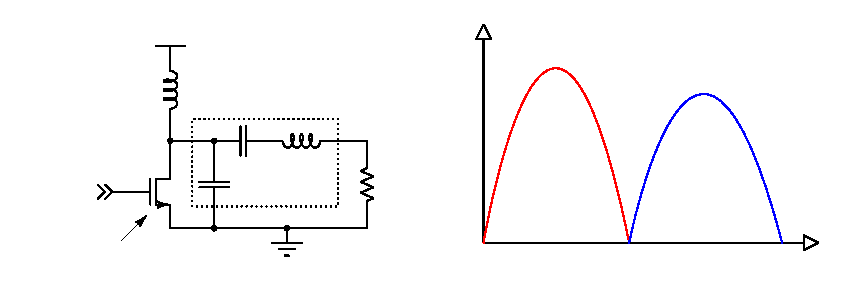
\includegraphics[scale=1.71644]{class-e-op}\\
   % translate x=345 y=905 scale 0.22
   \putbox{2.09in}{2.26in}{1.20}{Amplifier Output}%
   \putbox{2.43in}{2.01in}{1.20}{Network}%
   \putbox{1.01in}{2.09in}{1.20}{RFC}%
   \putbox{0.09in}{1.09in}{1.20}{Gate}%
   \putbox{0.09in}{0.84in}{1.20}{Drive}%
   \putbox{0.59in}{0.18in}{1.20}{Gate Drive}%
   \putbox{4.18in}{1.09in}{1.20}{Load}%
   \putbox{6.01in}{2.59in}{1.20}{Vds}%
   \putbox{7.68in}{2.34in}{1.20}{Id}%
   \putbox{6.76in}{0.09in}{1.20}{Time}%
   \putbox{1.59in}{2.84in}{1.20}{48V}%
   } % close 'parbox'
   } % close 'scalebox'
   \vspace{-\baselineskip} % this is not necessary, but looks better
